\documentclass[12pt]{article}
\usepackage{geometry}                % See geometry.pdf to learn the layout options. There are lots.
\geometry{letterpaper}                   % ... or a4paper or a5paper or ... 
%\geometry{landscape}                % Activate for for rotated page geometry
\usepackage[parfill]{parskip}    % Activate to begin paragraphs with an empty line rather than an indent
\usepackage{daves,fancyhdr,natbib,graphicx,dcolumn,amsmath,lastpage,url}
\usepackage{amsmath,amssymb,epstopdf,longtable}
\usepackage{paralist} 
\DeclareGraphicsRule{.tif}{png}{.png}{`convert #1 `dirname #1`/`basename #1 .tif`.png}
\pagestyle{fancy}
\lhead{CE 3372 -- Water Systems Design}
\rhead{FALL 2017}
%\rhead{FALL 2010}
%\rhead{SPRING 2011}
%\rhead{FALL 2011}
%\rhead{SPRING 2012}
%\rhead{FALL 2013}
%\rhead{FALL 2016}
%\rhead{SPRING 2017}
%\lfoot{EXERCISE 1 -- REVISION 1}
%\lfoot{EXERCISE 1 -- REVISION 2}
%\lfoot{EXERCISE 1 -- REVISION 3}
\lfoot{ES 18}
\cfoot{}
\rfoot{Page \thepage\ of \pageref{LastPage}}
\renewcommand\headrulewidth{0pt}



\begin{document}
\begin{center}
{\textbf{{ CE 3372 -- Water Systems Design} \\ {Exercise Set 18}}}
\end{center}

%\begingroup
%\begin{tabular}{p{2in} p{4.5in}}
Purpose: Develop expertise in application of Gradually Varied Flow equation in Open Channel Flow\\
%%~ & ~ \\
%%ABET General Criteria 3: & (a) \dots apply knowledge of mathematics, science, and engineering  \\
%%~ & (e)  \dots solve engineering problems  \\
%%~ & (k) \dots an ability to use the techniques, skills, and modern engineering tools necessary for engineering practice. \\
%%%~ & ~ \\
%%%Grading Criteria:  & Completion; Correct Solutions; Calculation Details \\
%\end{tabular}
%\endgroup
\section*{\small{Exercises}}
\begin{enumerate}
%%%%%%%%%%%%%%%%%%
\item Water flows at a steady rate of 192$ft^3/s$ through a concrete-lined rectangular channel 16 ft wide as depicted in Figure \ref{fig:channel_profile}. The water enters the $0.35 \%$ sloped channel ($S_0 = 0.0035$) at location $1$ and is flowing at $110\%$ normal depth ($1.1 \times y_n$).  The water exits over a 3-foot tall weir (assume sharp-crest weir) at location $2$.\footnote{The water-surface-profile spreadsheet on the class server can be adapted to this problem, or you can create your own.}

\begin{figure}[htbp] %  figure placement: here, top, bottom, or page
   \centering
   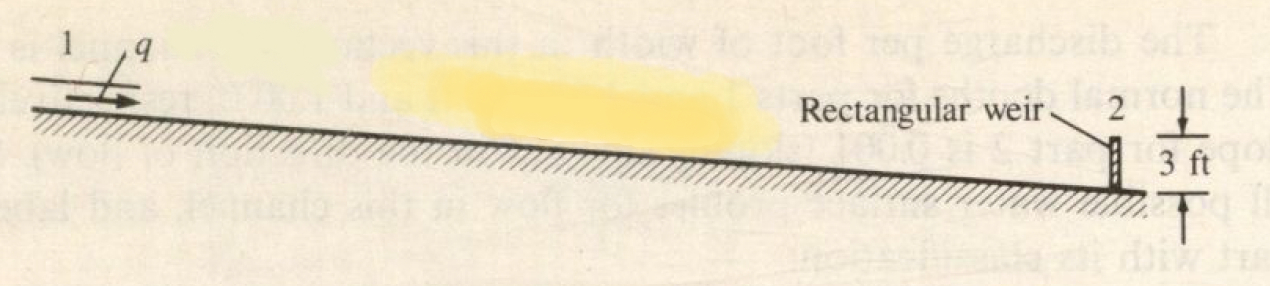
\includegraphics[width=6in]{channel_profile.jpg} 
   \caption{Profile of concrete-lined rectangular channel.}
   \label{fig:channel_profile}
\end{figure}

Determine: 
\begin{enumerate}[i]
\item The critical depth for the channel (in feet).
\item Assuming flow over the weir must pass through critical depth, what is the pool depth just upstream of the weir? (Hint: Add the critical depth to the weir height as an approximation to the pool depth)
\item Using the variable-step method, determine the water-surface profile from location $2$ to location $1$.
\item How far upstream from the weir is the flow at $110\%$ normal depth? (i.e. how far upstream is location $1$ from location $2$.
\item What is the average $\Delta x$ in your computations if the $\Delta y$ is $0.1$ feet?
%\item Include sample calculations (if you use a spreadsheet, screen capture a portion of the calculations section).
\item Include a plot of the water surface elevation, and the channel bottom elevation (a profile plot -- like the figure, but with the horizontal distance as the x-axis).
\end{enumerate}
%
%\item Repeat the problem, except model the situation in SWMM.
%\begin{enumerate}[i]
%\item Make your SWMM model have conduits that are the average $\Delta x$ from the problem above.
%\item Include a screen capture of your SWMM model showing the computed water-surface-profile.   
%\end{enumerate}
%\clearpage
%\item Estimate the peak flow of a square shaped 50 acre, single family residential area in Harris County. 
%The site is graded from an elevation of 150ft at the corner to 139ft at the outlet as depicted on Figure \ref{fig:watershed.jpg}.
%
%\begin{figure}[h!] %  figure placement: here, top, bottom, or page
%   \centering
%   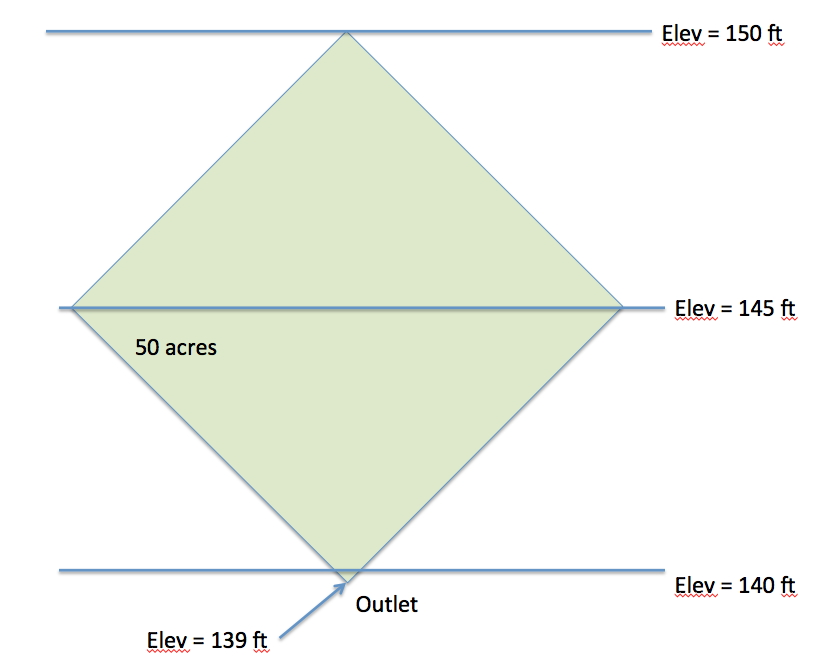
\includegraphics[width=4in]{watershed.jpg} 
%   \caption{50 acre square watershed with elevation contour overlay}
%   \label{fig:watershed.jpg}
%\end{figure} 
%
%\begin{enumerate}[i)]
%\item Draw on the diagram the longest flow path from the highest elevation to the outlet, and determine the length of the flow path in feet.
%\item Estimate the time of concentration.
%\item Estimate the peak discharge for a 10-year, 6-hour storm using the Rational Method.
%\item Use SWMM to simulate the runoff hydrograph from the watershed for a 10-year, 6-hour storm using the NRCS 6-hr Rainfall Distribution Curves (in Lecture Notes).  Include a screen capture of the SWMM model.
%\item Include a screen capture of the sub-catchment dialog box where you supply sub-catchment area, and width.   Describe how you selected your width for your model.   
%\item Determine the calculated peak discharge from the SWMM model and compare its value to the value from the Rational Method.
%\end{enumerate}
%
%%\item A grass-lined roadside swale (ditch) is to be built as a trapezoidal channel to carry 20 cubic-feet per second, with a 1 foot freeboard.   If the desired flow depth is 1 foot, and the right of way available to fit the ditch is 12 feet, what is the required side slope and bottom width.   The longitudinal slope is 1\%.
%%\begin{enumerate}[i]
%%\item Sketch the cross section and label the width, depth, and side slope.
%%\item Write the appropriate relationships between velocity, depth, and discharge for the section.
%%\item Compute the required side-slope in the section.
%%\item Compute the mean section velocity in the section.
%%\end{enumerate}

\end{enumerate}
\end{document}  